\documentclass[11pt,twoside]{book}
\setcounter{secnumdepth}{3}
\setcounter{tocdepth}{3}
\usepackage{graphics}

\makeatletter

\pagestyle{headings}
\usepackage[dvips]{graphicx}

\title{LDS Users Guide}
\author{Chris Debenham}
\date{Version 1.2}


\makeatother
\begin{document}
\maketitle
\tableofcontents{}


%
% NEW CHAPTER FOR INTRODUCTION
%

\chapter{Introduction}


\section{What is LDS?}

LDS stands for Lyric Display System.\\
 It is a computer-based replacement for the overheads used to display
song lyrics in events such as church services.


\section{Who was LDS written for?}

LDS was originally written for use at Gosford Baptist Church in Gosford,
Australia.\\
 It was designed for use in Churches and so has features specific
to Church usage.


\section{Who was this guide written for?}

This guide has been written for people who wish to use LDS and assumes
that LDS has already been installed and is in a working state.\\
 It's target audience is the average non-technical user.



%
% NEW CHAPTER FOR USING LDS
%

\chapter{Using LDS}


\section{Starting the Interface and Server}

Starting the interface way vary depending on how LDS has been setup.\\
A good idea is to place an icon on the desktop of your first screen
which when clicked runs  \emph{/usr/bin/lyric\_interface.pl }%
\footnote{default installation location, change if you installed it somewhere else
}\\
To load the server part just go to the Applications menu and chose
Lyric Server.


\section{The Main Interface}

Once the main interface has been loaded up you will see a screen similar
to figure \ref{figure:interface} on page \pageref{figure:interface}.

{ \begin{figure}
\caption{\label{figure:interface}Main Interface}
\resizebox*{1\textwidth}{!}{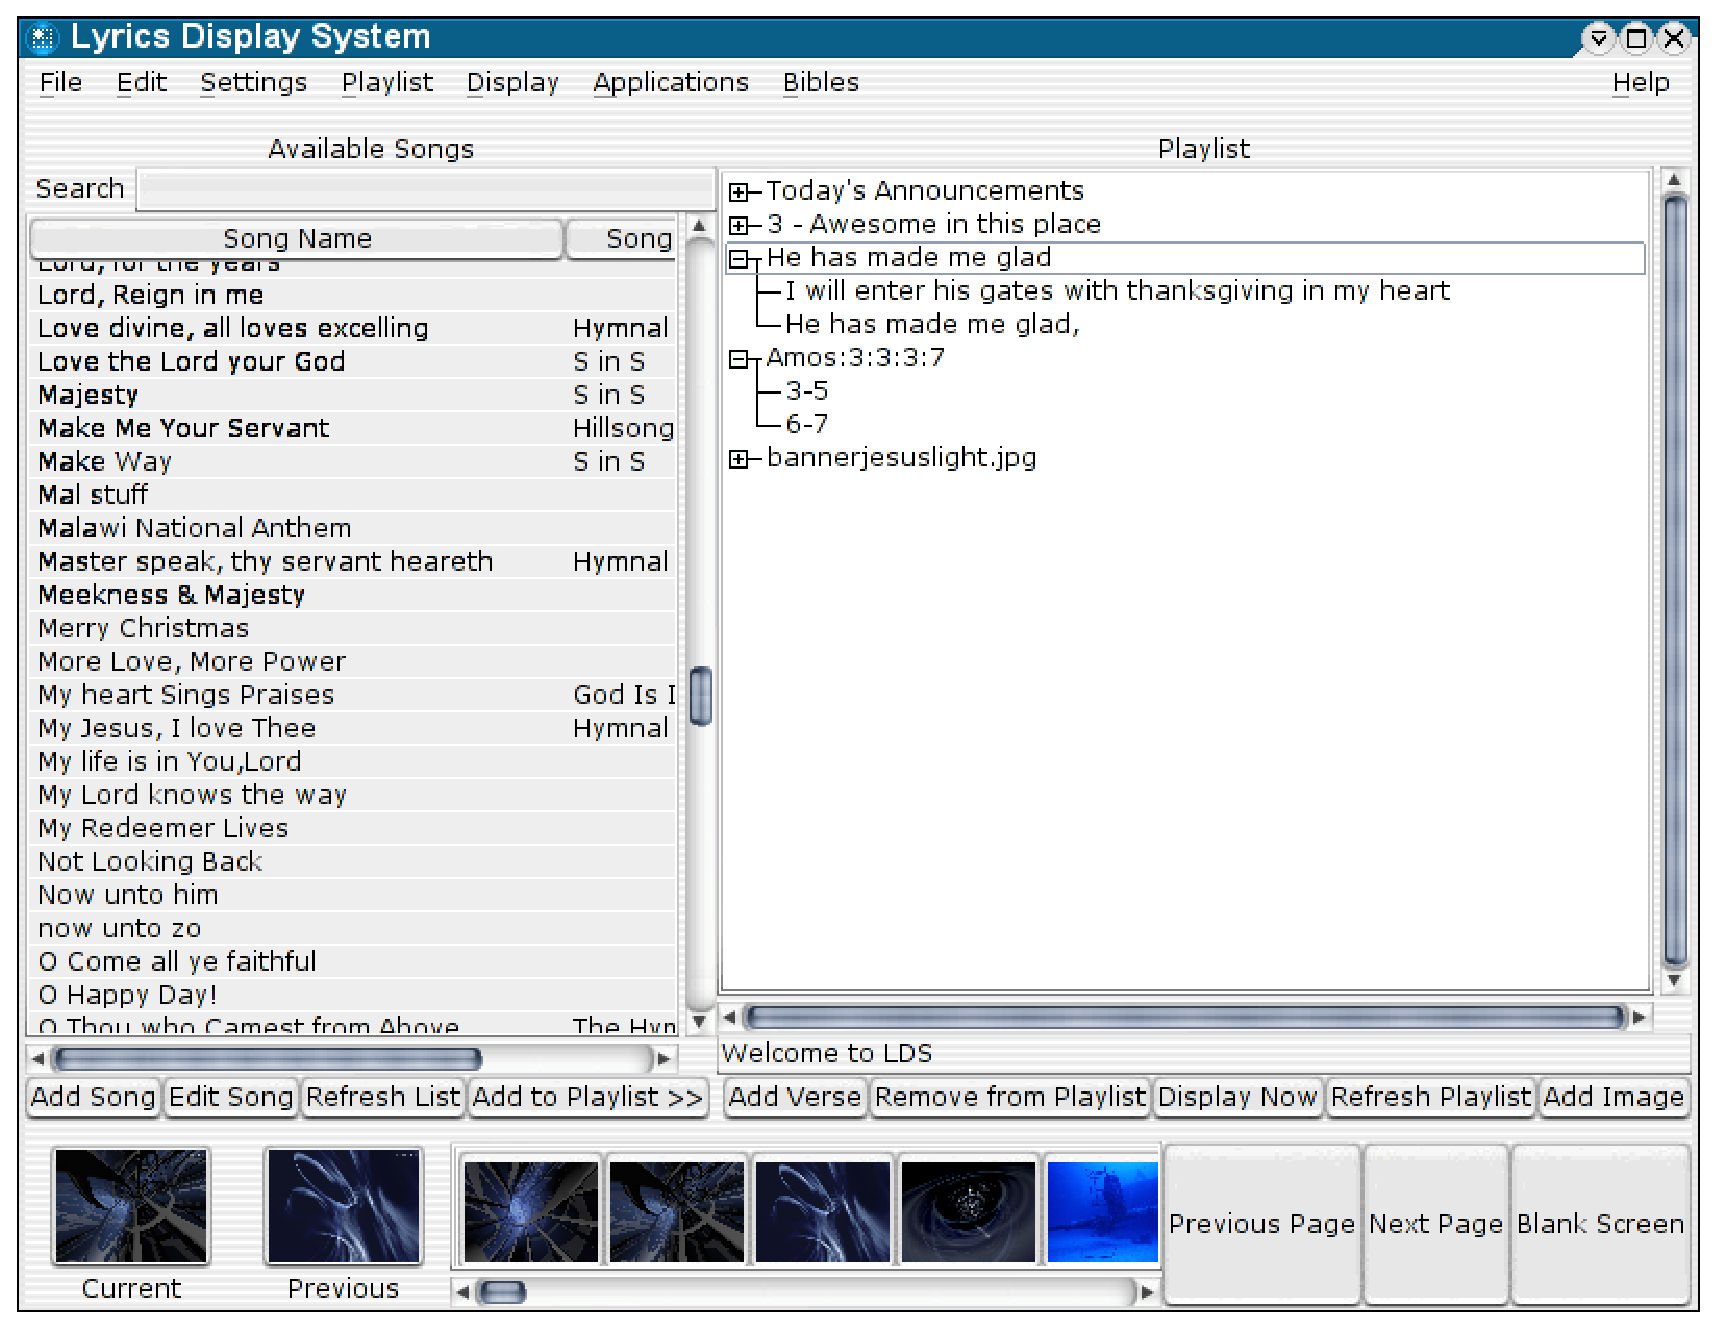
\includegraphics{interface.eps}}
\end{figure}
/par}

\subsection{Menus}
	Menus are available at the top of the interface window and can be used to perform a range of tasks.
	\begin{description}
		\item[File]
		Standard File menu
		\begin{description}
			\item[Exit] Exit the interface
		\end{description}
		
		\item[Edit]
		Actions performed on playlist/songlist
		\begin{description}
			\item[Add Song] Add a song to the available songs
			\item[Advanced Search] Search for a song by its lyrics
			\item[Edit Song] Edit the song currently selected in the songlist
			\item[Delete Song] Delete the song currently selected in the songlist
			\item[Refresh List] Refresh the songlist
		\end{description}

		\item[Settings]
		LDS Server settings
		\begin{description}
			\item[Select Main Font] Select the font that will be used for the main text (lyrics)
			\item[Select Header Font] Select the font that will be used for the song name
			\item[Select Footer Font] Select the font that will be used for the song artist
			\item[Select Font Colour] Select the font colour
			\item[Select Background Image] Select the background image from a dialog box
		\end{description}

		\item[Playlist]
		Actions performed on playlist
		\begin{description}
			\item[Add to Playlist] Add the song currently selected in the songlist to the playlist
			\item[Remove from Playlist] Remove the song currently selected in the playlist from the playlist
			\item[Clear Playlist] Clear the entire playlist (useful at start of service)
			\item[Refresh Playlist] Refresh the playlist (in case changes have been made to song names, lyrics etc this will reflect them in the playlist)
			\item[Add Verse] Add verses to the playlist
			\item[Add Presentation] Add a presentation to the playlist - not complete
		\end{description}
	
		\item[Display]
		Commands to send to server
		\begin{description}
			\item[Previous Page] Display the previous page in the current song
			\item[Next Page] Display the next page in the current song
			\item[Display Now] Display the page currently selected in the playlist
		\end{description}

		\item[Applications]
		Run external applications on second screen\\
		This is configurable in the \emph{lds.conf} file, two examples are given.
		\begin{description}
			\item[Lyric Server] Load the lyric server on your second screen
			\item[Xterm] Load an xterm on the second screen (provided as an example on how to add applications to this menu
		\end{description}

		\item[Bibles]
		Choose the bible translation used by the interface/server to display verses
		\begin{description}
			\item[King James Version] Display bible verses from the King James Version
		\end{description}

		\item[Help]
		Get help
		\begin{description}
			\item[About] About this program
		\end{description}

	\end{description}


\subsection{Songlist/Playlist Area}
	The songlist/playlist area encompasses the list of available songs on the left of the interface window, the playlist on the right and the search area at the top-left.
	\begin{description}
		\item[Search area] Enter text here and the available songs will show songs containing that text in their title
		\item[Available songs] This is a list of all available songs (possibly only those matching search text)\\
			You can drag items from this list to the playlist area and they will be added to the playlist.\\
			Right-clicking on the list pops up a menu of relevant menuitems (see Menu section for description of items).\
		\item[Playlist]
			The playlist area shows the current playlist as a tree of items.\\
			Each first-level item is a song/verse/image/presentation.\\
			Clicking on the plus sign beside an item will expand it and show the pages contained within it.\\
			Double-clicking on an item, or sub-item will display that page/song on the server immediately.\\
			Right-clicking on the list pops up a menu of relevant menuitems (see Menu section for description of items).\
	\end{description}

\subsection{Buttons}
	\begin{description}
		\item[Add Song] Add a song to the available songs
		\item[Edit Song] Edit the song currently selected in the songlist
		\item[Refresh List]Refresh the songlist
		\item[Add To Playlist]Add the song currently selected in the songlist to the playlist
		\item[Add Verse]Add verses to the playlist
		\item[Remove From Playlist] Remove the song currently selected in the playlist from the playlist
		\item[Display Now] Display the page currently selected in the playlist
		\item[Refresh Playlist] Refresh the playlist (in case changes have been made to song names, lyrics etc this will reflect them in the playlist)
		\item[Add Image] Adds an image from the lds/images folder
		\item[Previous Page] Tells the server to display the previous page in the current song
		\item[Next Page] Tells the server to display the next page in the current song
		\item[Blank Page] Remove all text from the server display (will leave backgroung image on screen
	\end{description}

\subsection{Backgrounds}
	This encompasses the two images on the bottom left and the image area beside it
	\begin{description}
		\item[Current Image] Show what the current background image is
		\item[Previous Image] Shows what the previous background image was. Click on it to make it the current background
		\item[Available Images] Show a thumbnail list of available background images
	\end{description}


\section{Introducing the Server}

	The server is just a single large window that is designed to take up the full screen and be projected to the congregation.\\
	\\
	The Background is set initially by the configuration file and can then be changed by the interface.\\
	\\
	At the top is the page title which will be the song name or bible verse if provided.  The font is controlled by \emph{header font}.\\
	\\
	In the middle is the main text area. This contains the lyrics of the song or the contents of the bible verse. The font is controlled by \emph{main font}.\\
	\\
	At the bottom is the page footer which will be the song artist or bible verse if provided.  The font is controlled by \emph{footer font}.\\
	\\
	Pressing Up/Down/Left/Right while the server is focussed will tell it to go to the next/previous song or next/previous page\\


\section{The Add/Edit Song Window}

This window is used to add/edit songs.  Once it has loaded up you will see a screen similar to figure \ref{figure:add} on page \pageref{figure:add}.

{ \begin{figure}
\caption{\label{figure:add}Add/Edit Window}
\resizebox*{1\textwidth}{!}{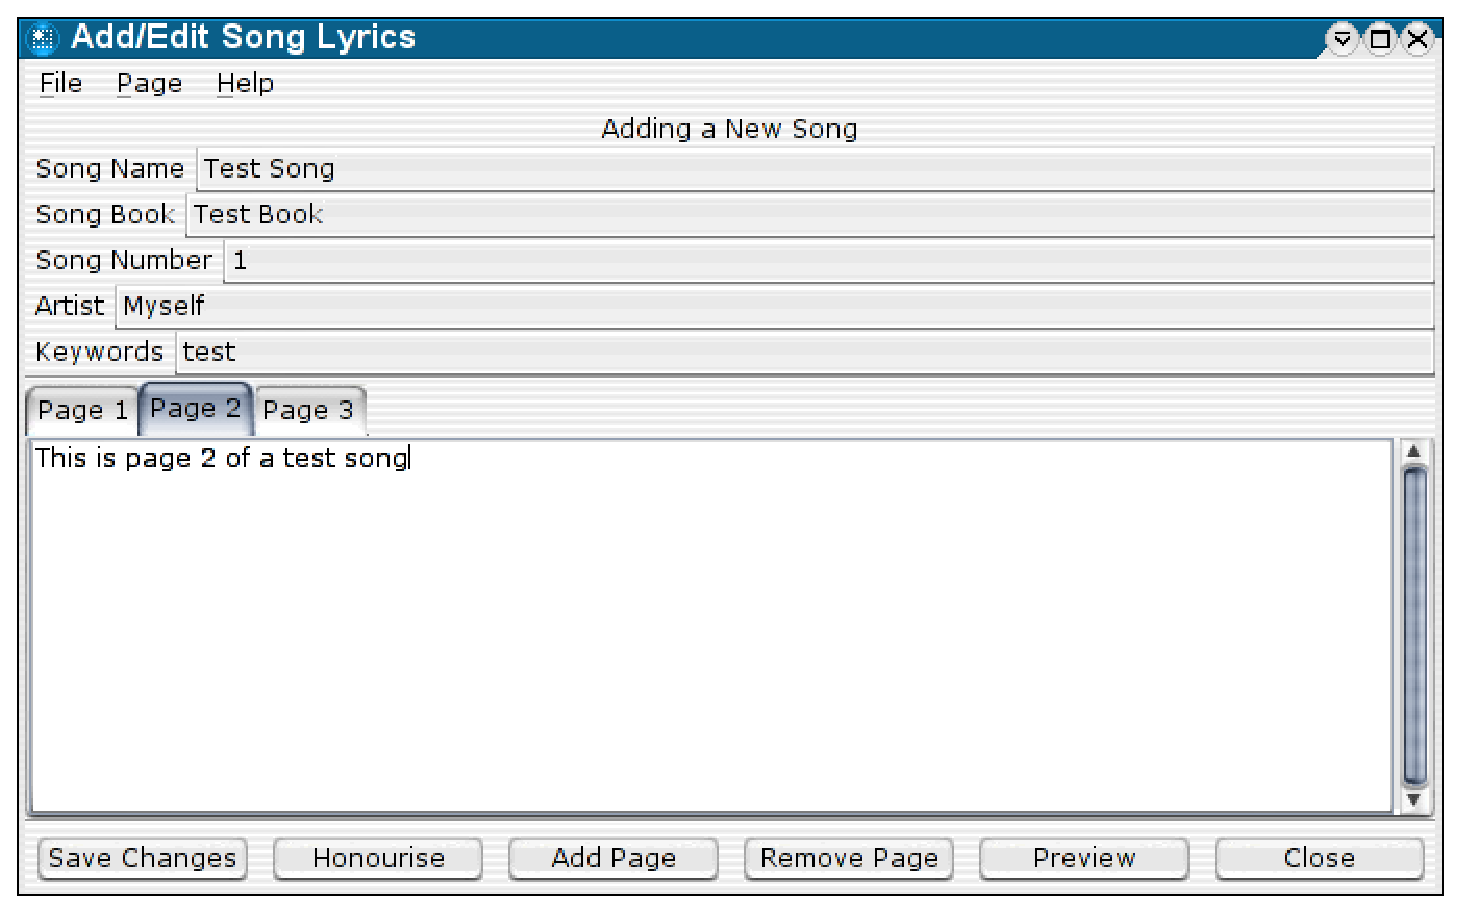
\includegraphics{addedit.eps}}
\end{figure}
/par}

\subsection{Menus}
	Menus are available at the top of the window and can be used to perform a range of tasks.
	\begin{description}
		\item[File]
		Standard File menu
		\begin{description}
			\item[Import] Import a song from a file, opens a file dialog to choose your file from
			\item[Export] Export a song to a file, opens a file dialog to choose where to save the song to
			\item[Save] Saves the current song and closes the window
			\item[Exit] Exit the window
		\end{description}
		\item[Page]
		Page operations
		\begin{description}
			\item[Add Page] Add a new blank page after the current page
			\item[Remove Page] Remove the current page
			\item[Preview Page] Preview the current page in the server screen
		\end{description}
		\item[Help]
		Help options
		\begin{description}
			\item[About] About this program
		\end{description}
	\end{description}

\subsection{Buttons}
	The buttons down the bottom provide the same operations as the menus and one extra
	\begin{description}
		\item[Save Changes] Saves the current song and closes the window
		\item[Honourise] Capitalizes important words such as God, Jesus etc.
		\item[Add Page] Add a new blank page after the current page
		\item[Remove Page] Remove the current page
		\item[Preview] Preview the current page in the server screen
		\item[Close] Closes the current window \emph{without saving}
	\end{description}

\subsection{Editing Area}
	The editing area contains a text area and a number of tabs.\\
	Each tab refers to a page (the page number is stated in the tab name)\\
	Changing pages is done by clicking on the relevant tab.\\

%
% NEW CHAPTER FOR HOWTOS
%

\chapter{HOW-TOs}

\section{Add a song to the playlist}
Adding a song to the playlist can be done is a variety of ways.\\
You can drag a song from the \emph{available songs} list to the playlist or select a song from the \emph{available songs} list then choose \emph{Add to Playlist} from either the right-click menu, the buttons down the bottom or the \emph{Playlist} menu

\section{Add a song to the system}
First choose \emph{Add Song} from the menu or the click the button.\\
This will bring up a new window which you can use to edit/create songs.\\
See the Section about the Add/edit window for details

\section{Add a verse}
Click on the \emph{Add Verse} button or choose it from the menu.

\section{Add background images}
To add background images simply place the image file in \emph{/usr/share/lds/backgrounds}\footnote{default installation location, change if you installed it somewhere elses} then load up the interface (or restart it if it is already loaded.

\section{Add images for use as playlist items}
To add images simply place the image file in \emph{/usr/share/lds/images}\footnote{default installation location, change if you installed it somewhere elses} then load up the interface (or restart it if it is already loaded.

\section{Change Fonts/Colours}
Choose one of the options from the \emph{Settings} menu

\section{Change the song background}
Click on any of the images at the bottom of the interface to set the current background.  You can also choose \emph{Change Background} from the menus

\section{Delete a song from the system}
Select the song in the available songlist then choose \emph{Delete Song} from the right-click menu, the top menu or click on the \emph{Delete Song} button.

\section{Display a particular page}
Double-click on the page in the playlist to display immediately (changes current song as well as page)

\section{Display a song}
Double-click on the song title in the playlist or double-click the first page in the song.\\
You can also select the first page/song title then click the \emph{Display Now} button.

\section{Display the next/previous page}
Choose from the menu or click on the relevant buttons down the bottom-right of the interface.

\section{Edit a song in the system}
Select the song in the available songlist then choose \emph{Edit Song} from the menu, right-click menu or buttons.\\
Editing proceeds along the same lines as adding a song but the system automatically fills out the details from the song.

\section{Remove a song from the playlist}
Select the song in the songlist and click \emph{Delete Song} from the menu, right-click menu or buttons.

\section{Run external commands}
External applications are available from the \emph{Applications} menu and anything from that menu will be run on your second display.\\
To edit/add/remove items from this edit your /etc/lds.conf.

\end{document}
